\section{Spannungsregler}

% % % % % % % % % % % % % % % % % % % %
% %Lineare Spannungsregler
% % % % % % % % % % % % % % % % % % % %
	\subsection{Lineare Spannungsregler} 
		Für alle linearen Spannungsregler gilt: $ P_{V}=(V_{E}-V_{a}) \cdot I_{a} $\\
		Einsatz für geringer Spannungsunterschied zwischen Eingangsspannung und der
		geregelten Ausgangsspannung \\
% % % % % % % % % % % % % % % % % % % %
% %Qualitätsmasse
% % % % % % % % % % % % % % % % % % % %		
	\subsection{Qualitätsmasse}
		relativer Stabiliersungsfaktor: $S' = \dfrac{\Delta U_e/U_e}{\Delta U_a/U_a}$\newline
		Temperaturkoeffizient: $TK_u = \dfrac{1}{U_a}\dfrac{dU_a}{dT}$\\
		Lastabhängigkeit: $r_a = \dfrac{dU_a}{dI_a}$
% % % % % % % % % % % % % % % % % % % %
% %Spannungsregler mit Längstransistor
% % % % % % % % % % % % % % % % % % % %
\subsection{Spannungsteiler mit Längstransistor}
 	\begin{minipage}{200pt}
		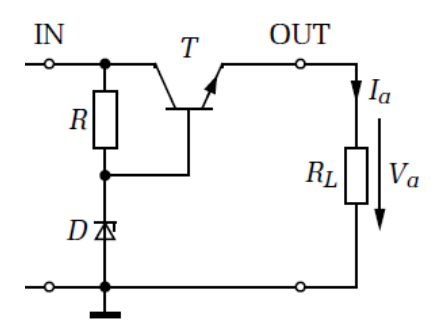
\includegraphics[width = 5cm]{./images/spgregler/01_laengstransistor} 
 	\end{minipage}
	\begin{minipage}{300pt}
	\begin{tabular}{p{120pt}p{170pt}}
	$U_{A}=U_{Z}-U_{BE}$ &
	$R_{V}=\dfrac{U_{E}-U_{Z}}{I_{Z}+I_{B}}$\\
	$I_{B}=\dfrac{I_{C}}{B}$&
	$I_{C} \approx I_E = I_L $\\
	$R_{i}\approx\frac{r_{Z}}{\beta} $&
	\\
	\hline
	$U_{Z}$: Z-Dioden-Spannung&
	$I_{Z}$: Strom durch die Z-Diode\\
	$R_{i}$: Innenwiderstand der Schaltung &
	$r_{Z}$: dyn. Innenwiderstand der Z-Diode\\
	$B$: Gleichstromverstärkung &
	$\beta$: Dynamische Verstärkung \\
	\end{tabular}
	\end{minipage}\\
% % % % % % % % % % % % % % % % % % % %
% %Spannungsteiler mit Opamp
% % % % % % % % % % % % % % % % % % % %
\subsection{Spannungsregler mit Opamp}
	\begin{minipage}{200pt}
		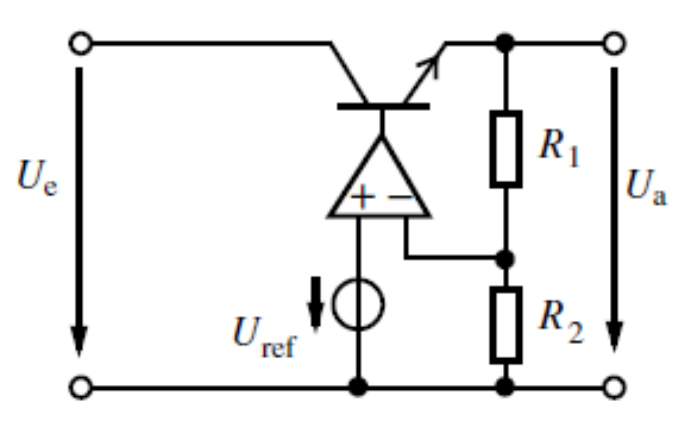
\includegraphics[width = 5cm]{./images/spgregler/02_spgregler_opamp.png}
	\end{minipage}
	\begin{minipage}{300pt}
			$V_{out} = V_{ref}\cdot\dfrac{R_2+R_1}{R_2}$\\
			Low-Dropout-Regler (LDO): PMOS-FET anstatt Transistor.
	\end{minipage}\\




